
%%!TEX root = ./heapvis.tex

\section{Case Studies}

We now present the results of visualizing data structures in several Java
programs and use these as a basis for discussion of Heapviz's strengths and
weaknesses.  First, we show three constructed examples built using standard 
Java container classes.  Second, we explore two real-world benchmarks,
\_209\_db~\cite{specjvm98} and SPEC JBB 2000~\cite{specjbb2000}.

\subsection{Constructed Examples}

We first consider three examples constructed from standard data structures 
from the Java class library.  In the first example, Heapviz reveals a 
difficult-to-find performance bug in a hash table with little effort on the 
user's part.  In the second example, the user takes advantage of Heapviz's 
interactive abilities to explore the effect of insertion order on the
structure of a red-black tree.  In the final example, Heapviz's summarization
algorithm makes clear the sharing of elements contained in three distinct
data structures.

\subsubsection{Hash Table}

Hash tables are widely used in production software, and their average case 
time complexity is well understood by programmers. Furthermore, programmers
understand that using a poor hash function will cause too many elements to hash
into the same bin, resulting in $O(n)$ time complexity in the worst case.
But suppose a programmer is debugging a program that uses a hash table, and
she wants to determine whether that hashtable has elements distributed
evenly into bins. Using a debugger to do this would be extremely tedious,
and it would be difficult to instrument library hash table code.
Instead, we can use Heapviz to visualize the hash table and see whether
elements are evenly distributed among bins.

Figures~\ref{fig:goodhasher} and~\ref{fig:badhasher} show Heapviz 
visualizations of two different
Java \texttt{HashMap}s containing 100 elements each.  The \texttt{HashMap} in
Figure~\ref{fig:goodhasher} contains elements that use a good hash 
function, and the one in Figure~\ref{fig:badhasher}
contains elements that use a poor hash function.  We can clearly see 
in the bad \texttt{HashMap} that many elements have hashed into the same
bucket, and this has produced a long hash chain in that bucket.  Thus, if
the program performs an insert or lookup on an element that hashes into that 
bucket, it will pay an $O(n)$ cost instead of the expected $O(1)$ cost.
This is obvious from a glance at the Heapviz visualization.
Indeed, by examining the field values of the 
\texttt{HashMap\$Entry} objects in the long chain, the programmer can easily
determine which bucket is experiencing excess collisions and adjust the
hash function accordingly.

\begin{figure}
  \includegraphics[width=\textwidth]{figs/hashmap/goodhasher-simple.eps}
  \caption{A hash table with a good hashing function. The orange node is the 
  \texttt{HashMap} object, the large node at the center is the array of 
  buckets, and the red nodes on the perimeter are the internal 
  \texttt{HashMap\$Entry} objects used to implement the hash chains. 
  All the \texttt{HashMap\$Entry} nodes are a short distance
  from the array of buckets, indicating that the hash function has distributed
  keys evenly.}
  \label{fig:goodhasher}
\end{figure}

\begin{figure}
  \includegraphics[width=\textwidth]{figs/hashmap/badhasher-simple.eps}
  \caption{A hash table with a bad hashing function. As in 
  Figure~\ref{fig:goodhasher}, the orange node is the 
  \texttt{HashMap} object, the large node at the center is the array of 
  buckets, and the red nodes on the perimeter are the internal 
  \texttt{HashMap\$Entry} objects used to implement the hash chains. 
  One hash chain is much longer than the others, indicating an excess of
  collisions into that bucket.}
  \label{fig:badhasher}
\end{figure}

\subsubsection{Red-Black Tree}

A red-black tree is a type of self-balancing binary search tree that is
often used to implement a map data structure. To maintain the balanced 
property, a set of $tree rotations$ may be performed when inserting or 
removing a node from the tree.  In a red-black tree, internal tree nodes are
colored either red or black, and every path from a given node to a leaf
must contain the same number of black nodes. Thus, the worst case height 
of the tree is $2 \log n$, which occurs when all nodes are black except 
for those along one path of alternating red and black nodes.

Suppose a student wants to learn about red-black trees, specifically how
to construct a tree in both the best and worst cases.  It would be 
impractical to examine manually a reasonably-sized tree using a debugger, 
but a visualization of the tree with the nodes colored appropriately would 
make it obvious whether we have a ``good'' or ``bad'' tree. Heapviz's 
interactive tools make it easy to create such a visualization.

Below, we list the five steps a Heapviz user would perform
to transform an unsummarized heap graph into an effective diagram of the 
contained red-black tree. A figure accompanies each step, and our 
supplemental video demonstrates this procedure.  The process takes no more 
than 90 seconds for an experienced user.

\begin{enumerate}

\item The user loads the graph into Heapviz. Default colors are assigned 
to connected subgraphs to make separating them easier. Notice the main 
graph component separating into two subsections. (Figure~\ref{fig:rb-1})

\item The user hides the components that aren't connected to the main component
to make navigation easier. She then hovers over the 
core of part of the graph, highlighting its neighbors. The connectedness 
of the tree and the highlighted \texttt{Integer} objects
tells us the tree's data is these \texttt{Integer}s. (Figure~\ref{fig:rb-2-2})

\item Being interested in only the structure of the tree, the user selects 
all the \texttt{Integer}s at once and hides them. Now, we see a central 
node of type \texttt{java.lang.Object} holding the graph together. 
Red-black tree leaf nodes may not contain 
data, and many implementations use a single sentinel node to mark all leaves.
The user deduces that this is the sentinel node and is not important
to the structure of the tree. (Figure~\ref{fig:rb-3})

\item The user hides the sentinel node, and the graph lays itself out.
Immediately the tree structure becomes obvious. Since all the nodes are 
the same class, the user has opted to use circles to represent nodes 
instead of labels to reduce clutter. (Figure~\ref{fig:rb-4-2})

\item With two simple queries and a few clicks, the user colors each 
internal node red or black according to a field value. Now the tree
looks like we would expect a red-black tree to look.
(Figure~\ref{fig:rb-5-2})

\end{enumerate}

Now that we can visualize a red-black tree, we can answer our question about
the best and worst cases.  Figure~\ref{fig:rb-5-2} shows a tree that was 
constructed by inserting keys in random order.  The red nodes are evenly 
distributed throughout the tree, and all paths from the root to a leaf
have approximately the same length---this is the best case. 
Figure~\ref{fig:rb-inorder} shows a tree that was constructed by inserting keys
in ascending order. The nodes in this tree are all black except for those along
one path in which nodes alternate between red and black. This is the worst 
case because the length of the alternating path is $2 \log n$, while all
the others are $\log n$.  Thus, by exploring with Heapviz we have learned 
that inserting keys in order produces the worst case red-black tree.

\begin{figure}
  \includegraphics[width=\textwidth]{figs/rbtree/rb-1.eps}
  \caption{The initial state of a Heapviz visualization of a red-black tree.
  Notice the main graph component separating into two subsections.}
  \label{fig:rb-1}
\end{figure}

\begin{figure}
  \includegraphics[width=\textwidth]{figs/rbtree/rb-2-2.eps}
  \caption{A Heapviz visualization of a red-black tree while a hover action
  highlights the immediate neighbors of the large \texttt{Integer} array
  at the center of the graph. This shows that the tree's data is in the
  \texttt{Integer}s.}
  \label{fig:rb-2-2}
\end{figure}

\begin{figure}
  \includegraphics[width=\textwidth]{figs/rbtree/rb-3.eps}
  \caption{A Heapviz visualization of a red-black tree after hiding the
  \texttt{Integer} objects (to focus on the structure of the tree). A single
  sentinel node of type \texttt{java.lang.Object} ties the graph together.}
  \label{fig:rb-3}
\end{figure}

\begin{figure}
  \includegraphics[width=\textwidth]{figs/rbtree/rb-4-2.eps}
  \caption{A Heapviz visualization of a red-black tree after hiding the
  sentinel node and setting the node display style to circles instead of
  labels. The tree structuyre is now obvious.}
  \label{fig:rb-4-2}
\end{figure}

\begin{figure}
  \includegraphics[width=\textwidth]{figs/rbtree/rb-5-2.eps}
  \caption{A Heapviz visualization of a red-black tree after coloring the
  nodes according to a field that indicates whether each node is red or
  black. Now the graph looks just as we would expect a red-black tree
  to look. Note that the red nodes are evenly distributed in the tree.
  This red-black tree was created by inserting keys in random order.}
  \label{fig:rb-5-2}
\end{figure}

\begin{figure}
  \includegraphics[width=\textwidth]{figs/rbtree/rb-inorder.eps}
  \caption{A Heapviz visualization of a red-black tree where keys were 
  inserted in ascending order. All nodes are black except for those along
  one path, where red and black nodes alternate---the worst case.}
  \label{fig:rb-inorder}
\end{figure}

\subsubsection{Overlapping Elements}
\label{overlap}

Consider a program that contains multiple data structures.  These data
structures each contain some subset of the data objects in the program,
and these subsets may overlap.  That is, of the objects in data structure 
$x$, some are pointed to only by $x$, some by $x$ and $y$, and some by 
$x$ and $z$.  Heapviz can explain this situation.

Figure~\ref{fig:complicated} shows
such a program.  This program has three data structures, a \texttt{TreeMap}, 
a \texttt{HashSet}, and a \texttt{LinkedList}, using the standard 
implementations in the Java class library.  These data structures contain
\texttt{IntBox} objects, some of which are shared by two or all three 
data structures.  The unsummarized graph on the left in 
Figure~\ref{fig:complicated} gives too much detail to discover this sharing, 
but the summarized graph makes the sharing
clear.  Each \texttt{IntBox} node in the summarized graph represents a set 
of concrete nodes with the same set of concrete predecessor nodes.  Thus 
the summarized graph explains the sharing of \texttt{IntBox} nodes among
the different data structures.  For example, we can see that the 
\texttt{IntBox} objects represented by node $a$ are pointed to only by
the \texttt{HashMap}, but the ones represented by nodes $c$ and $d$
are pointed to by both the \texttt{HashMap} and the \texttt{LinkedList}.
Thus we can determine that all \texttt{IntBox} objects in the 
\texttt{LinkedList} are also in the \texttt{HashMap}, but not all of the 
ones in the \texttt{HashMap} are in the \texttt{LinkedList}.  In the 
interactive visualization, the user can click on nodes to see exactly how many 
\texttt{IntBox} nodes are shared among the data structures, and how many are 
only in the \texttt{HashMap}.

From the nodes and edges in Figure~\ref{fig:complicated}, without looking 
at the source code of the program, we can determine that:
\begin{enumerate}
\item There are three data structures in the program: a \texttt{TreeMap}, 
a \texttt{HashSet}, and a \texttt{LinkedList}.
\item Each data structure contains objects of type \texttt{IntBox}.
\item Some \texttt{IntBox} objects (the ones represented by node $a$) are 
pointed to by only the \texttt{HashMap}.
The user could find the exact number by clicking on node $a$.
\item Some \texttt{IntBox} objects are shared by all three data structures
(node $c$), and others are shared by only two 
(nodes $b$ and
$d$).  Again, the exact number can be found by clicking on the appropriate 
summary node.
\item The \texttt{HashMap} contains all \texttt{IntBox} objects in the program.
The other data structures each contain a strict subset of the \texttt{IntBox}
objects.
\end{enumerate}

\noindent Heapviz makes clear the sharing among different data structures
without requiring the user to look at the program source code.

\begin{figure*}[t]
  \includegraphics[width=\textwidth]{figs/complicated}
  \caption{A Heapviz visualization of three data structures: a \texttt{TreeMap}, a
\texttt{HashSet}, and a \texttt{LinkedList}.  Each data structure contains a subset of
\texttt{IntBox} objects.  The unsummarized graph is on the left, and the summarized
graph is on the right.  Heapviz reveals the sharing among different data structures 
without requiring the user to look at the program source code.}
  \label{fig:complicated}
\end{figure*}

\subsection{Real Examples}

Now we assess Heapviz's visualization of two real-world benchmarks,
\_209\_db~\cite{specjvm98} and SPEC JBB 2000~\cite{specjbb2000}.  We
consider how Heapviz is successful in helping us understand the data structures
in \_209\_db and why it is less successful in summarizing the graph from SPEC
JBB 2000.

\subsubsection{\_209\_db}

%\begin{figure*}[t]
%  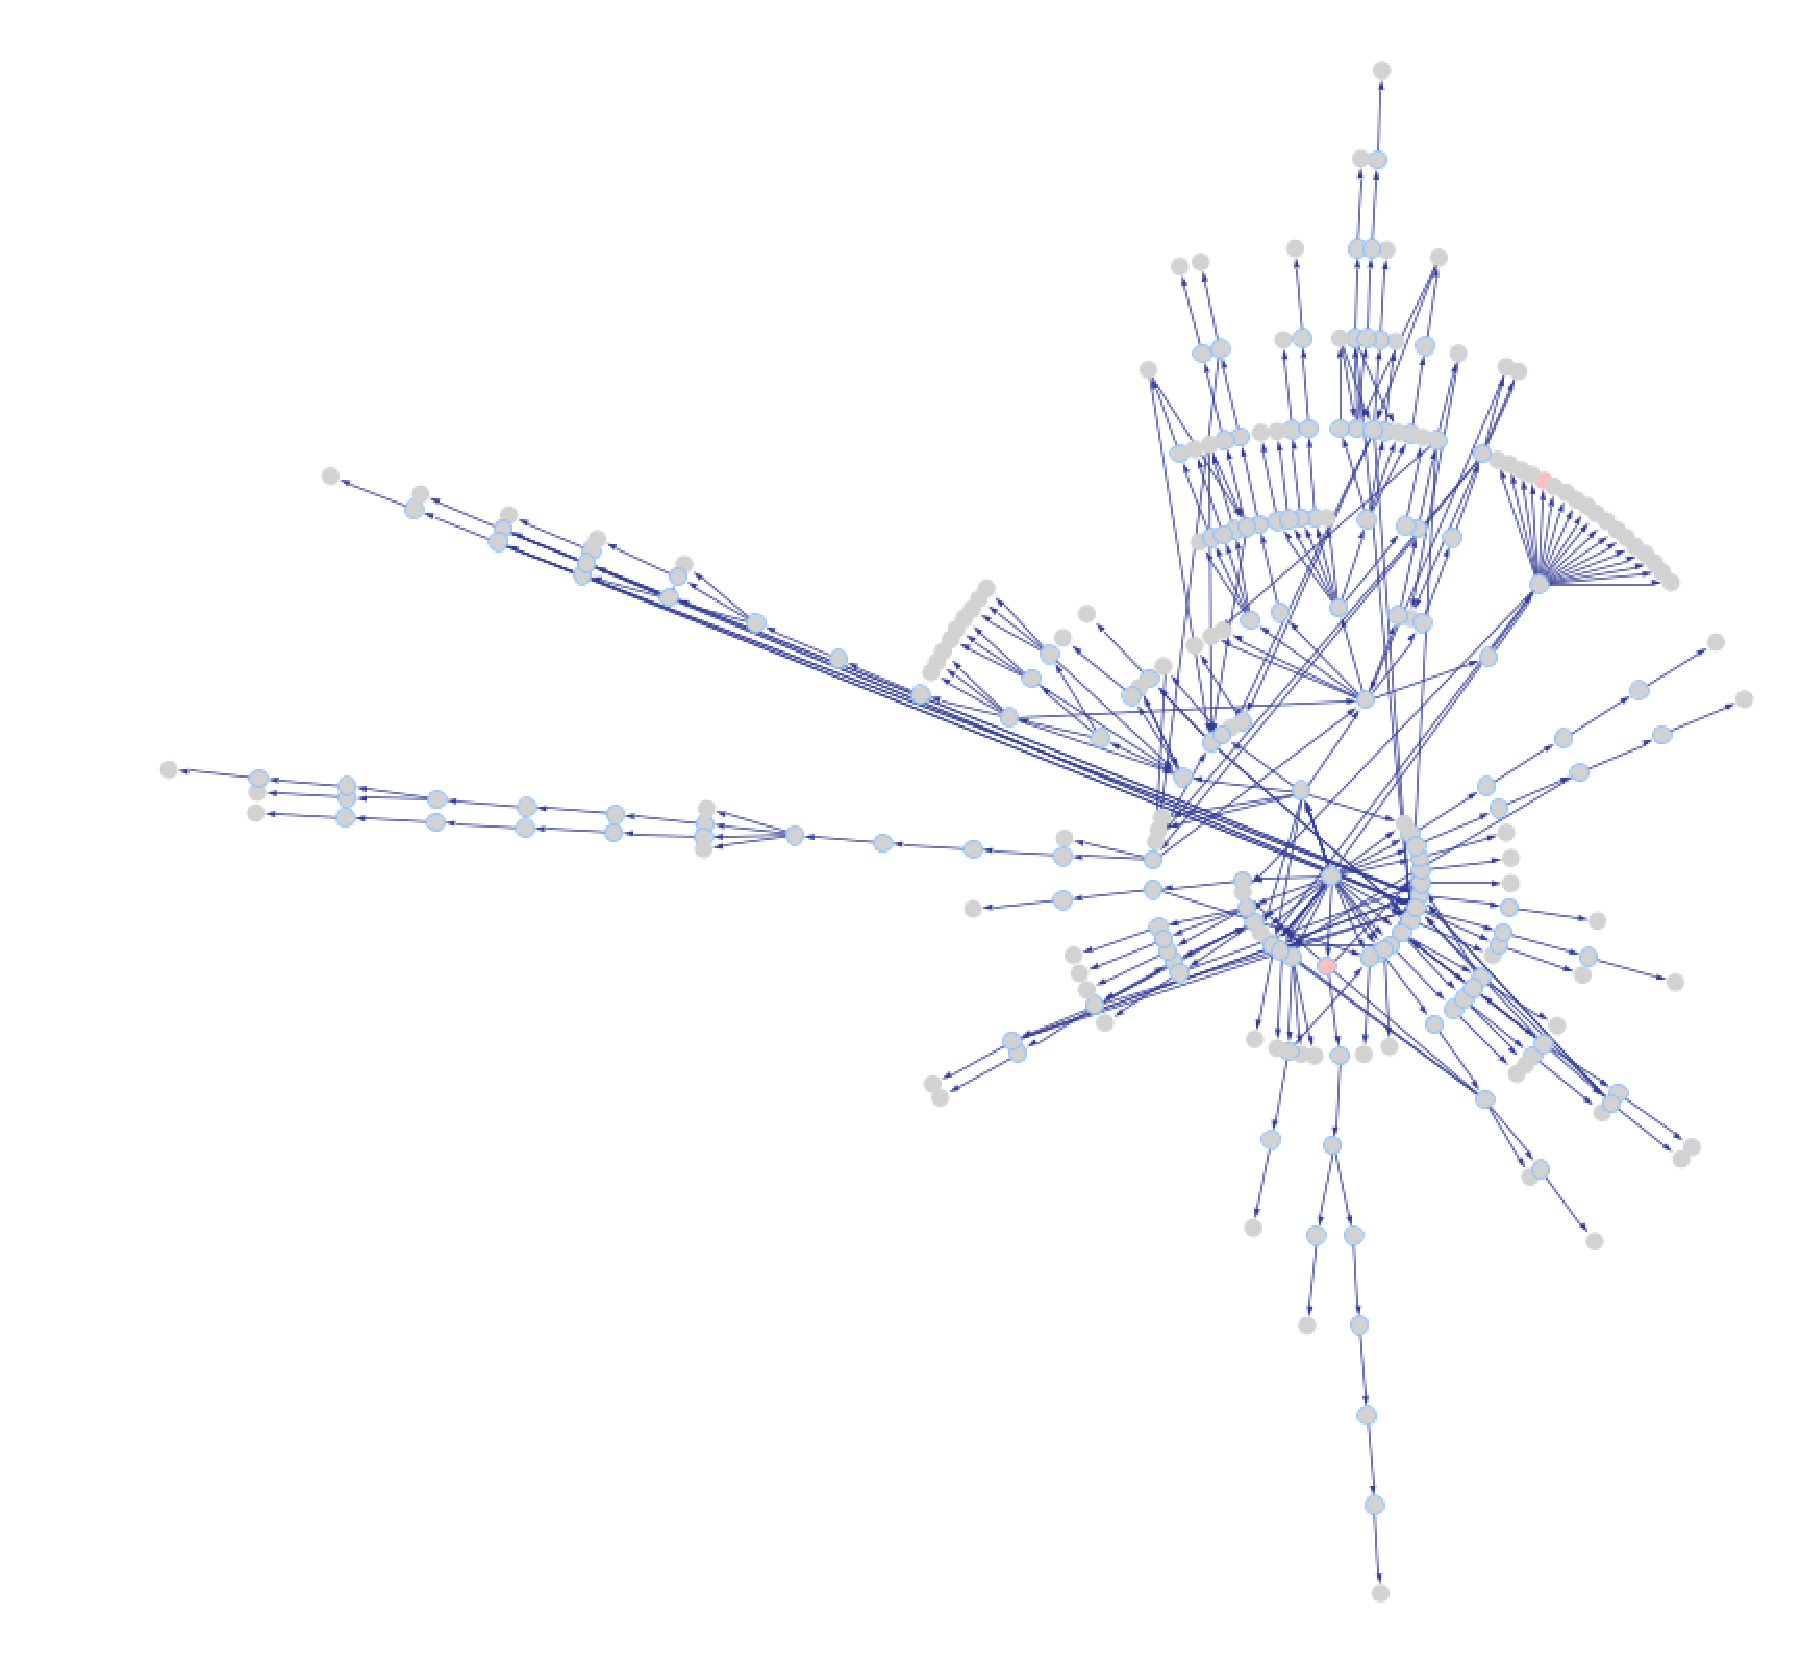
\includegraphics[width=0.85\textwidth]{figs/db}
%  \caption{A summarized visualization of the \_209\_db benchmark,
%which contains 294,002 objects in the concrete heap at this
%point in program execution. The summarized graph contains only 254 nodes and
%is comprehensible using the interactive visualization.}
%  \label{fig:db}
%\end{figure*}

\begin{figure*}[t]
  \includegraphics[width=\textwidth]{figs/db-zoomed-mod}
  \caption{A summarized visualization of the \_209\_db benchmark.  The 
bottom left shows the full graph, with the inset zoomed to 
show the program's primary data structure, a database.
This database contains two \texttt{Vector} objects, each containing 
strings or database entries. The node representing all entries in this 
database summarizes 15,332 nodes. Each database entry contain a 
\texttt{Vector} of strings; the total number of these strings in the 
database is 122,656.
}
  \label{fig:db-zoomed}
\end{figure*}

\_209\_db is a database benchmark from the SPEC JVM 98 benchmark
suite~\cite{specjvm98}.  It performs multiple database operations on an
in-memory database.  We took a heap snapshot of an execution of \_209\_db just
after the database is built from an input file and before any operations are
performed on the database.  Figure~\ref{fig:db-zoomed} shows the summarized
visualization on the bottom left, with the inset zoomed to show the program's
primary data structure.

Before summarization, the graph contained 294,002 objects; after 
summarization, it contained 254.  By zooming in on the nodes in the 
graph that summarize the most concrete
nodes,  we can see the primary data structure
in the program: an object of type \texttt{spec.benchmarks.\_209\_db.Database}.
This database contains two \texttt{Vector} objects (\texttt{Vector}s
are growable arrays of objects), which each contain 
strings or database entries.  The node that represents all database entries
in this database summarizes 15,332 nodes.  The database entries then each
contain a \texttt{Vector} of strings; the total number of these strings 
in the database is 122,656.  

By inspecting the source code of \_209\_db, we can explain what these data mean.
One of the two \texttt{Vector} objects pointed to by the database is used
to store a format string that describes the records included in each entry.
The other \texttt{Vector} holds the database entries.  Each database entry
uses a \texttt{Vector} to hold strings for each record: name, address, city,
state, and so on.  Though we had to look at the source code to understand 
this program, the visualization quickly showed us the primary data structure 
in the program and its high-level structure.

However, this example shows some of the limitations of Heapviz.  
Even though Heapviz was able to reduce the size of the graph by three orders
of magnitude, the graph is still somewhat large and difficult to understand 
at a glance.  In particular, it is difficult to pick out the important nodes in 
the graph, since nodes that summarize one concrete node are displayed the same
way as nodes that summarize many concrete nodes.  We discuss possible 
solutions to these issues in Section~\ref{future}.

% we provide ways to get rid of stuff we don't want, but maybe we should have
% ways to show only the stuff we do want

\subsubsection{SPEC JBB 2000}
\label{jbb}

\begin{figure}[t]
  \includegraphics[width=\columnwidth]{figs/jbb}
  \caption{A summarized visualization of the SPEC JBB 2000 benchmark, which 
contains 117,819 objects in the concrete heap at this point in program execution. 
The summarized graph contains 7578 nodes.  Although some large data structures 
are visible after this significant reduction, the graph is still cluttered.}
  \label{fig:jbb}
\end{figure}

The SPEC JBB 2000~\cite{specjbb2000} benchmark emulates a three-tier
client-server system, with the database replaced by an in-memory tree and
clients replaced by driver threads.  The system models a wholesale company,
with warehouses serving different districts and customers placing orders.  We
took a heap snapshot of SPEC JBB 2000 during the \texttt{destroy()} method of
the \texttt{District} class in order to understand the sharing of
\texttt{Order} objects stored by the \texttt{District}.  

A full visualization of the SPEC JBB 2000 heap snapshot is shown in
Figure~\ref{fig:jbb}.  From the 117,819 objects in the concrete heap at this
point in program execution, we produce a summarized graph of 7578 nodes, a
reduction of 93.5\%.  Although some large data structures are visible after
application of the summarization algorithm, the graph is still too 
visually complex.  
%\todo{AG: Is there any way to provide an estime of how much reduction the
%summarization provides in general?}

The characteristics of this data provide some clues as to limitations of the
summarization algorithm.  SPEC JBB 2000 represents an extreme form of the
simple program discussed in Section~\ref{overlap}, with a dense web of
connections among what we could consider the ``leaves'' of the data structures
-- objects that represent the individual elements of the program, such as
customers and orders.  In SPEC JBB, many of these ``leaves'' point to other
``leaves'' and have a one-to-one relationship.  This one-to-one pointer mapping
gives each of these ``leaves'' a unique predecessor set, preventing them from
being summarized.

For example, consider the \texttt{Order} objects in SPEC JBB.  An 
\texttt{Order} object points to the \texttt{Customer} who made that 
\texttt{Order}, and a \texttt{Customer} object points to the last 
\texttt{Order} the \texttt{Customer} made.  Thus, all \texttt{Customer}
objects point to different \texttt{Order} objects, which then point back
to the \texttt{Customer} object.  This situation is shown in 
Figure~\ref{fig:failure}.


Because \texttt{Customer} objects point to different \texttt{Order} objects,
any \texttt{Order} pointed to by a \texttt{Customer} has a unique predecessor
set and will not be merged with any other \texttt{Order}, unless the
\texttt{Customer} objects are merged first.  But because these \texttt{Order}
objects point back to different \texttt{Customer} objects, those
\texttt{Customer} objects also have unique predecessor sets and will not be
merged.  As a result, our algorithm cannot merge nodes that exhibit this
one-to-one structure.  We see this exact behavior in our graph: None of the
three hundred \texttt{Order} objects are summarized because each of them points
to and is pointed to by a different \texttt{Customer} object.  
We discuss possible solutions to this problem in Section~\ref{future}.

\subsection{HeapViz Summarizer}

\begin{figure}[t]
  \includegraphics[width=\columnwidth]{figs/summarizer}
  \caption{A summarized version of our HeapViz summarizer, after it produced
	   a summarized graph of our "Overlapping Elements" example.}
  \label{fig:summarizer}
\end{figure}


While working on HeapViz, we encountered some software problems. Amongst them: the
implementation of our summary algorithm was using too much memory. Having 
constructed a general debugging tool, and finding our selves needing to debug it,
we decided to use it on itself. So, we produced a heap snapshot of the 
summarizer working on our "Overlapping Elements" example in Section~\ref{overlap}.
The snap shot was
taken immediately after the summarizer generated the summarized graph. The
resulting visualization is shown in Figure~\ref{fig:summarizer}.

Since in this we are interested in the memory usage of the program, 
and minimzing it, it behooves us to look at types who's that have a large 
number of instances, and/or take up a large amount of memory. Examing the graph,
we can quickly find very large node of type \texttt{Value}, occupying 2.2 MB. Looking for other nodes of the same type, we discover another relatively
large one occupying 291 KB. 

Therefore, we conclude that reducing the size and/or number of \texttt{Value} objects will reduce memory usage. Examing the code for the Value class, we find this:

public class Value \{

  public Type type;

  private long objVal;
  private boolean boolVal;
  private char charVal;
  private float floatVal;
  private double doubleVal;
  private byte byteVal;
  private short shortVal;
  private int intVal;
  private long longVal;
  ...
\}

\texttt{Value} is being used to represent various Java values; here it is
essentially being used as a tagged union type; sometimes it reprsents a
object value, sometimes and boolean value, etc. and which kind of value 
it is representing is signified by the \texttt{type} field. However, suppose
particular \texttt{Value} instace is representing a object value, it still
has fields for a boolean value,  char value, a float value, and etc. In this case,
that would mean using 38 bytes of memory, while only 8 bytes are required. With
our heap containing 58,456 instances of type \texttt{Value} this is a lot of over head. 

Thus, we refactored the \texttt{Value} class into an abstract parent class \texttt{Value} and subclasses for each kind of value, each containing only the necessary fields. Re-running the summarizer on the refactored version itself results in~\ref{fig:summarizer-post}. Here we can see that \texttt{Value} has been broken up into
several concrete subclasses, and by probing the nodes we can quickly determine
that all of these instances use 177 KB (down from over 2 MB). 


\begin{figure}[t]
  \includegraphics[width=\columnwidth]{figs/summarizer-post}
  \caption{A summarized version of our HeapViz summarizer, after it produced
	   a summarized graph of our "Overlapping Elements" example,
	   post refactoring}
  \label{fig:summarizer-post}
\end{figure}

 



